\begin{frame}{State Machine}
\begin{center}
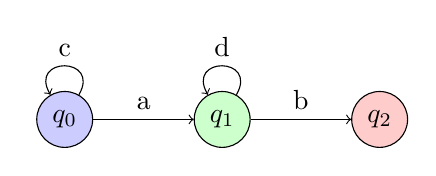
\begin{tikzpicture}[node distance=2cm]
    \node[circle, draw, fill=blue!20] (q0) {$q_0$};
    \node[circle, draw, fill=green!20, right of=q0] (q1) {$q_1$};
    \node[circle, draw, fill=red!20, right of=q1] (q2) {$q_2$};
    
    \draw[->] (q0) -- node[above] {a} (q1);
    \draw[->] (q1) -- node[above] {b} (q2);
    \draw[->] (q0) to[out=60,in=120,looseness=4] node[above] {c} (q0);
    \draw[->] (q1) to[out=60,in=120,looseness=4] node[above] {d} (q1);
\end{tikzpicture}
\end{center}

\footnotesize
\texttt{\textbackslash draw[->] (q0) to[out=60,in=120,looseness=4] node[above] \{c\} (q0);}
\end{frame}